%----------------------------------------------------------------------------------------
%	Debug options
%----------------------------------------------------------------------------------------
% chktex-file 2
% chktex-file 8
% chktex-file 11
% chktex-file 13
% chktex-file 18
% chktex-file 36
% chktex-file 39
% chktex-file 44
%----------------------------------------------------------------------------------------
\chapter{Results and discussion}\label{cha:Discussion}
% # Why does this section matter?
% # How does it reflect on investigating the gap in Scrum
% # Transition to the next section
% Synthesize the findings in literature and method
% Derrive findings from that
Through the synthesis of findings from the literature review and the \gls{methodology} used in this thesis, this chapter aims to provide a comprehensive understanding of the challenges faced by Scrum practitioners.

The chapter is structured into four main sections, each of which focuses on a different aspect of the investigation. The first section, \fancyref{sec:Findingsfromdatacollection}, presents the results of the empirical data collected through the \gls{methodology} used in this thesis.

The second section, \fancyref{sec:Comparisonofresultswithpreviousstudies}, compares the findings of this investigation with those of previous studies on the topic. This comparison provides a nuanced understanding of the challenges faced by Scrum practitioners and how they have evolved over time.

The third section, \fancyref{sec:Interpretationoftheresults}, provides an in-depth interpretation of the findings from the data collection and comparison with previous studies. This section highlights the key challenges faced by Scrum practitioners and how they impact the implementation of the \gls{methodology}.

Finally, the fourth section, \fancyref{sec:Implicationsoftheresults}, discusses the practical implications of the findings for Scrum practitioners and organizations. This section provides recommendations in form of \glspl{guideline} for how organizations can overcome the challenges faced in implementing Scrum and how future research can address the gaps identified in this investigation.

In summary, this chapter provides a comprehensive understanding of the gap between the theory and practice of Scrum by synthesizing the findings from both the literature and \gls{methodology}.

\section{Results from data collection}\label{sec:Findingsfromdatacollection}
This section is a crucial aspect of this chapter as it presents the results of the empirical data collected through the \gls{methodology} used in this thesis. This section highlights the findings of the primary research conducted to explore the gap between the theory and practice of Scrum. The results presented in this section provide a deep insight into the challenges faced by Scrum practitioners and organizations in implementing the \gls{methodology} effectively.

This section will lay the foundation for the subsequent sections, where the findings will be compared with previous studies, interpreted, and discussed in terms of their implications. In this section, the findings are presented in a clear and concise manner, providing a comprehensive overview of the results of the research.

The composition of the businesses represented among the interviewees in this study was analyzed. 25\% of the businesses were classified as Microenterprises and 25\% as Small Businesses. Medium enterprises accounted for only 8.33\% while Large enterprises represented 41.67\%. 

In terms of \gls{agile} \glspl{methodology}, Scrum was utilized by 58.33\% of the businesses, a Hybrid approach combining Scrum and Waterfall was used by 16.67\%, \ac{safe} by 16.67\% and 8.33\% employed the adapted \ac{less} \gls{methodology}. A notable observation was that 40\% of the Large enterprises in the study utilized the \ac{safe} \gls{framework}.

The results of this study provide insights into the utilization of the Scrum \gls{framework}. According to the data, approximately 48.57\% of the surveyed individuals adhere to the textbook definition of Scrum. The average duration of a Scrum Sprint was determined to be 1.57 weeks, with 41.7\% of the interviewees indicating that they employ a two-week Sprint. 

The average team experience with Scrum was found to be 3 years, while the average personal experience with the \gls{framework} was 7 years. This should be sufficient for a team to notice the problems they face and for an individual to be able to reflect on the maturity of the organization and their integration.

35\% of the teams utilizing Scrum reported having received some form of training, while 50\% of the interviewees using the \gls{framework} indicated that they have read the Scrum Guide. The most widely referenced version of the Scrum Guide was found to be the 2013 edition, with versions from 2011 and 2020 tied for second place. 

Approximately 42.86\% of the Scrum users held a certificate from a company or organization, with 100\% of the \ac{safe} users holding a certificate for either Scrum or \ac{safe}. The Scrum users believed that holding a certificate offered more expertise compared to not holding one, while \ac{safe} users believed it provided only a minimal increase in knowledge beyond the basics. Neither group believed that holding a certificate made someone an expert in their role or the \gls{framework}. 

With regards to \glspl{transformation}, 33.33\% were accompanied by \gls{agile} coaches, 25\% were accompanied by \acp{pm}, and a smaller proportion, less than 25\%, were executed solely by the team.

In terms of integration success, Scrum users rated their success at 76.79\%, while Hybrid users rated their success at 62.5\% and \ac{safe} users at 56.25\%. The individual utilizing the adapted \ac{less} \gls{framework} reported a successful integration. 

The products developed by the interviewees encompass web-based solutions for \glspl{client}, software development, and a variety of services. An analysis of the responses provided by Scrum users revealed that 28.57\% of them perceived their approach to be insufficient for their product, with variability noted across different projects. However, none of the interviewees expressed that their approach was inappropriate for their product. 

An examination of the four \glspl{framework} revealed that the average self-assessment for self-management among Hybrid users was the lowest at 60\%, with Scrum users exhibiting the second lowest average at 68.57\%. 

The average motivation for Scrum users to switch to a different \gls{framework} was found to be the lowest, at 37.14\%, in comparison to Hybrid or \ac{safe} users. The user of the adapted \ac{less} \gls{framework} demonstrated the lowest average motivation for a change, at 20\%, when compared to the average of the other three \glspl{framework}.

\begin{figure}[!ht]
	\begin{center}
        \makebox[\textwidth]{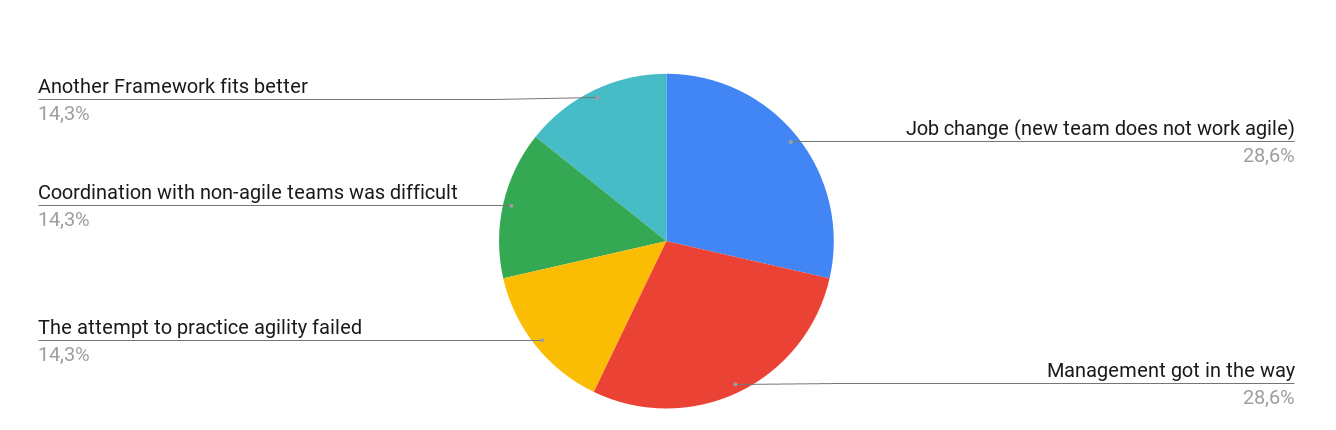
\includegraphics[width=\textwidth]{./assets/images/reasons-to-change.png}}
        \caption{Reasons to change to a different framework other than Scrum}\label{fig:reasons-to-change}
    \end{center}
\end{figure}

The Figure~\ref{fig:reasons-to-change} visualizes the most picked options for the Scrum practitioners. 

28.6\% of the respondents stated that they would move away from the Scrum \gls{framework} due to a job change or that their management got in the way of their Scrum integration. 14.3\% stated that other reasons for a change in their \gls{methodology} would be another better fitting \gls{framework}, difficult coordination with non-agile teams or that their attempt to practice agility failed

Of the 12 participants interviewed, not all provided answers to the question of which departments within their organizations utilize Scrum. However, among those who did provide answers, it was reported that 100\% of the development department employed Scrum. Additionally, among the Scrum users, 50\% of the project management department and 25\% of the \ac{ui} and \ac{ux} department utilized Scrum. 

The data shows that, among the organizations that use Scrum, 86\% on average reported using Daily Scrums, Sprint Reviews, and Backlog Refinements. On average, 71\% reported using Retrospectives and Sprint Plannings. 57\% reported using a digital Kanban board, while 43\% reported using User Stories, Story Points, and Planning Poker. The usage of alignment and control \glspl{method}, such as the Definition of Ready and Done, was reported by 14\% of the Scrum-using organizations.

Organizations of the medium size reported the highest usage of these \gls{agile} \glspl{method}, followed by small businesses, and then large organizations. Microenterprises reported the lowest usage.

The results of this study indicate that small and medium-sized organizations experience fewer difficulties in integrating Scrum compared to microenterprises and large enterprises. On average, small and medium-sized organizations reported encountering 8 out of the 38 potential issues associated with the integration process, as identified in the relevant literature. In contrast, microenterprises and large enterprises reported encountering 23.5 of the 38 potential difficulties on average. 

The most frequently reported problems with Scrum as a \gls{framework} among the interviewees were: (1) resistance from management to relinquish control; (2) lack of experienced personnel; (3) a large number of stakeholders; and (4) limitations on the influence of \gls{agile} coaches and Scrum masters imposed by management (reported by 29\% of interviewees on average). Other Problems are represented in Figure~\ref{fig:problems-with-scrum}.

\begin{figure}[!ht]
	\begin{center}
        \makebox[\textwidth]{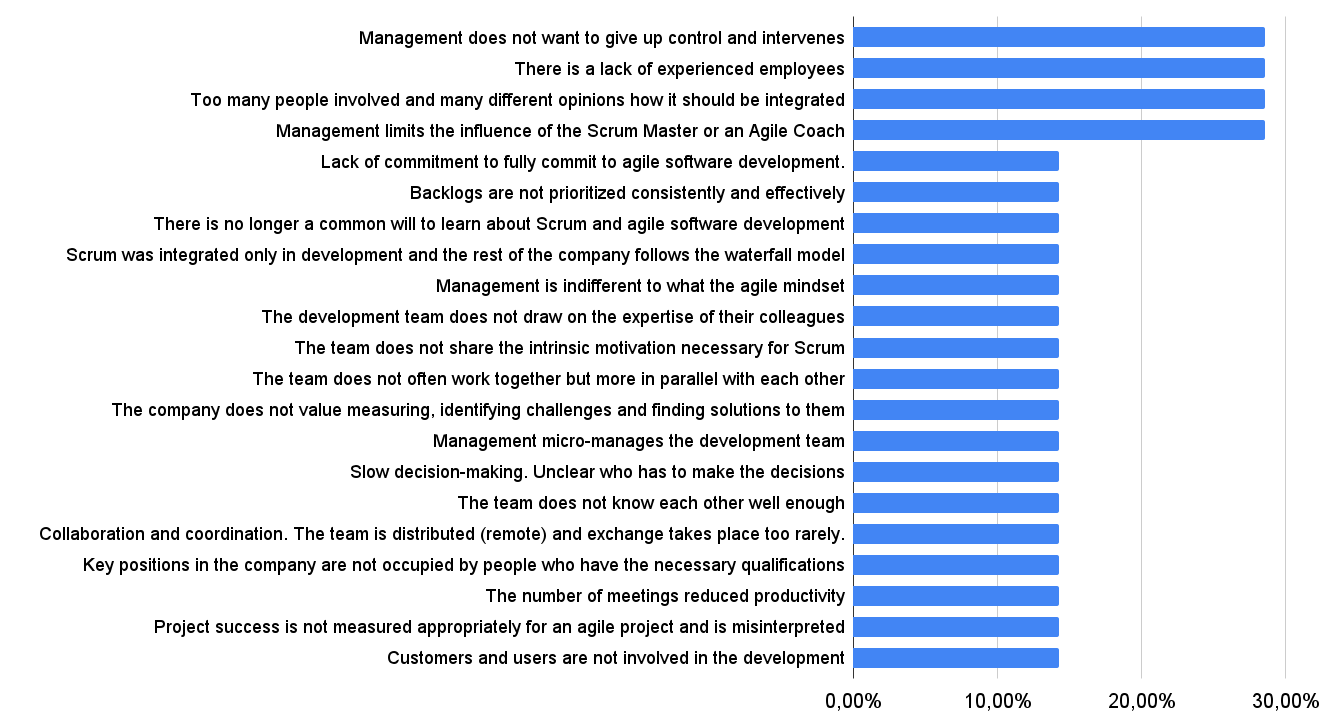
\includegraphics[width=\textwidth]{./assets/images/problems-with-scrum.png}}
        \caption{Reported average frequency of problems with Scrum}\label{fig:problems-with-scrum}
    \end{center}
\end{figure}

The results of this study suggest that a common approach to address difficulties encountered during the integration of \ac{asd} and the Scrum \gls{framework} is through training. Approximately 57\% of the respondents reported that training in \ac{asd} and the Scrum \gls{framework} was the most tried solution. Additionally, 43\% reported that training in feedback and communication culture was also a solution attempted, which indicates further challenges with the \gls{adoption} of new cultural beliefs within the organization. Yet, 57\% may still be too low as the respondents still reported problems with their \gls{adoption} related to lack of alignment and common beliefs.

To address the difficulties encountered, 43\% of the respondents reported trying the Scrum \gls{framework} for a certain period of time and following the Scrum Guide closely. Another 43\% reported solutions such as transparent communication of strategic and operational goals by management and utilizing Daily Scrums for efficient planning and coordination, which seems to be the logical solution to problems in this direction.

However, 29\% of the respondents reported not using demos and product increments for \gls{customer} and \gls{client} testing. Another 29\% reported that they had management support in writing for their \gls{adoption}, but only 14\% reported that middle management had learned new tasks and relinquished control.

Approximately 71\% of the interviewees using Scrum as their \gls{framework} reported not incorporating Concept Sprints with \glspl{client} for upfront design and planning, furthermore reducing the benefits of collaboratively working together with \glspl{client} on-site. This reinforces the widely held view that Scrum lacks design and planning upfront. Additionally, none of the interviewees utilizing Scrum as their \gls{framework} reported utilizing dedicated Enhancement Sprints.

Among the \glspl{framework}, including Scrum, the Hybrid of Scrum and Waterfall, and \ac{safe}, the Interviewees utilizing Scrum reported on average the most benefits (6 out of 8). Small businesses and medium-sized enterprises reported the most benefits from their \gls{adoption} of the Scrum \gls{framework}, and this trend was also observed with the \gls{adoption} of any new \gls{framework} different from Scrum. 

Approximately 71.43\% of the Scrum practitioners reported improved predictability, transparency, and visibility, aligning with the key goals of the Scrum \gls{framework}. Additionally, 57.14\% reported reduced risks and enhanced teamwork, which may indicate that \ac{asd} aligns with human collaboration and thinking processes. 42.86\% reported enhancements in effectiveness, productivity, team morale, product quality, and \gls{client} satisfaction, which are common outcomes associated with \ac{asd}, as validated by the findings of this study. Furthermore, 42.86\% reported the utilization of faster feedback from real users, which may have led to improved product quality and \gls{client} satisfaction.

\section{Comparison of results with previous studies}\label{sec:Comparisonofresultswithpreviousstudies}
This section provides a nuanced understanding of the challenges faced by Scrum practitioners by comparing the findings of this investigation with those of previous studies on the topic. The comparison of results with previous studies provides a more complete picture of the gap between the theory and practice of Scrum and enables a deeper understanding of the current state of the field.

The comparison in this section not only highlights the similarities and differences between the results of this investigation and previous studies, but also sheds light on the unique contributions of this study. The results of the comparison provide a solid basis for the interpretation of the findings and help to establish the significance of this study in the larger context of research on the topic.

\subsection*{Deviations and Challenges}\label{subsec:DeviationsandChallenges}
This study expands upon the existing literature on the implementation of the Scrum \gls{methodology} by showcasing deviations from the prescribed Sprint \gls{methodology} detailed in the Scrum Guide. The study findings reveal an average Sprint length of 1.57 weeks and 41.7\% of respondents utilizing 2-week Sprints. However, the study departs from previous research, as described in section~\fancyref{subsubsec:UnderstandingSprints}, by not finding the use of dedicated Enhancement Sprints~\cite[p.~2]{Sutherland2005Fos}. The current study offers valuable insight by suggesting that organizations considering the \gls{adoption} of Scrum should experiment with the \gls{framework} before making any alterations~\cite[pp.~9--13]{Wang2018Taa}, as also described in section~\fancyref{subsec:DiscussionTheoryPracticeGap}.

\subsection*{Limited Departmental Participation}\label{subsec:LimitedDepartmentalParticipation}
The study presents empirical evidence that supports prior research by disclosing that the majority of participants report that the development department is the primary user of Scrum, with limited involvement from other departments~\cite[p.~233]{Rubin2012ESA}, as previously discussed in section~\fancyref{subsubsec:TransformingTheMethodology}.

Moreover, the study extends the current body of literature by indicating a correlation between the success of Scrum implementation, the number of challenges faced, organizational culture, and the degree of participation from departments outside of development such as management~\cite[p.~125]{Moreira2013AtA}, which was also mentioned in section~\fancyref{subsubsec:TransformingManagement}.

\subsection*{Low Engagement}\label{subsec:LowEngagement}
This study provides further support for the prevalent belief that there is limited engagement with the Scrum \gls{methodology} among the participants and their teams. This aligns with previous research highlighting the need for comprehensive training and shared understanding of the \gls{methodology}~\cite[p.~72]{Maximini2018ISi}, found in section~\fancyref{subsubsec:BudgetingTrainging}. The study also adds to the existing literature by indicating that variations in the \glspl{guideline} prescribed within the Scrum Guide may result in different interpretations within teams. Additionally, the data highlights the significance of external expertise, as none of the participants considered certification as a marker of expertise in their role or the \gls{framework}, which partially confirms the hypothesis from section~\fancyref{subsubsec:DeviationOfRoles}, that Scrum Masters lack expertise and therefore \gls{agile} coaches with experience get hired.

\subsection*{Challenges in Client Collaboration}\label{subsec:ChallengesinClientCollaboration}
The study provides empirical evidence that supports previous research conclusions regarding the limited participation of \glspl{client} in organizations implementing Scrum, leading to difficulties in collaboration. Section~\fancyref{subsubsec:SellingScrum} stated the criticality of the involvement of the \gls{client} in the development process~\cite[p.~5]{Coyle2009Acs}.

\subsection*{Adoption and Success Across Organizational Size and Maturity}\label{subsec:AdoptionSuccessOrganizationalSize}
This study confirms prior research findings that larger enterprises tend to adopt scaling \glspl{framework}~\cite[p.~50]{Moreira2013AtA} and extends these findings by suggesting that simple \glspl{framework} such as Scrum may be easier to implement compared to complex systems like \ac{safe}, confirming former research~\cite[p.~119]{Gall1986SHs} presented by section~\fancyref{subsubsec:ChoosingAFramework}. The study also presents evidence of a positive correlation between the use of \gls{agile} \glspl{method}, lower problems, and greater benefits among small to medium-sized organizations. However, it is essential to note that further investigation is necessary to thoroughly evaluate the cultural differences that may exist between different organization sizes.

\subsection*{Adoption and Evolution of the Scrum Framework}\label{subsec:AdoptionEvolutionScrum}
The present study concurs with prior research in that the majority of Scrum practitioners are still predominantly from software development departments. However, this study also observes a growing trend of Scrum \gls{adoption} in non-software departments~\cite[Revision 2010--2013]{Schwaber2020SGR} as described in section~\fancyref{subsec:historyOfScrum}.

This study supports the prior findings, described in section~\fancyref{subsubsec:EmbracingSelfManagement}, that hybrid approaches to Scrum tend to yield low self-assessment scores in terms of self-management~\cite[p.~24]{Koning2019AT}, although it departs from existing literature by revealing that Scrum itself exhibits similarly low levels of self-management. The study further confirms the significance of management in the successful \gls{adoption} of a new \gls{framework}~(\citeNP[p.~125]{Moreira2013AtA};~\citeNP[pp.~37--38]{Boehm2005Mct}), in accordance with previous studies found in section~\fancyref{subsubsec:TransformingManagement}. The study contributes to the existing body of knowledge by uncovering a limited utilization of alignment \glspl{method} as prescribed by the Scrum guide, despite their potential to enhance collaboration and effectiveness.

\section{Interpretation of the results}\label{sec:Interpretationoftheresults}
This section provides an in-depth understanding of the gap between the theory and practice of Scrum. Through an analysis of the findings from the data collection and comparison with previous studies, this section highlights the key challenges faced by Scrum practitioners and how they impact the implementation of the \gls{methodology}.

This section goes beyond simply presenting the results and provides an in-depth examination of the findings to understand the underlying causes and effects of the challenges faced by Scrum practitioners. In this section, the results are not only presented but also analyzed and interpreted to provide a deeper understanding of the key challenges faced by Scrum practitioners.

The interpretation of the results provides a basis for the discussion of the practical implications of the findings, which is presented in the subsequent section.

The findings of this study are consistent with prior research that highlights the need for extensive training and shared understanding in the implementation of Scrum. This study also supports the notion that smaller and medium-sized organizations may be more flexible in adapting to new \glspl{methodology}. However, further investigation is needed to fully evaluate any cultural differences between organizations of different sizes. The low levels of self-organization within organizations utilizing Scrum suggest challenges in integrating the culture, while reduced \gls{client} involvement in testing processes indicate issues with client-collaboration. This study also confirms the critical role of management in the \gls{adoption} of new \glspl{framework} and the impact of uneven distribution and \gls{commitment} to the culture on participation from other departments.

This study extends the existing body of knowledge by examining the impact of different versions of the Scrum Guide on the integration of Scrum. The results suggest that variations in the Scrum Guide may lead to different understandings, making it a factor to consider. The study also found that organizations heavily rely on external experts, implying a need for more internal investment in training and building expertise. Deviations from the Sprint \gls{methodology} may reflect conscious change management decisions or difficulties in transitioning to Scrum. Further research is needed to fully assess the impact of Sprint length. The study highlights the value of organizations conducting their own research and avoiding unthinking adherence to \glspl{framework}.

\newpage

The findings of this study diverge from previous research that found simpler \glspl{framework} to be easier to implement with fewer difficulties compared to complex \glspl{framework}. The discrepancy between the results may be due to differences in \gls{methodology} or sample population. Although the latest revision of the Scrum Guide has aimed to simplify the \gls{framework}, the study suggests that more clarification is needed regarding alignment \glspl{method} and strategies for successful \gls{adaptation}. Further research is necessary to reconcile conflicting results and determine the root causes of the discrepancy.

The results of this study challenge prior research that found close collaboration to be a significant benefit of Scrum. This study found that the level of testing and collaboration with \glspl{client} was lower than expected, indicating that Scrum and \ac{asd} are often utilized as process enhancements rather than full cultural shifts. Further research is needed to reconcile this contradiction and establish a more accurate understanding of the topic.

\section{Implications of the results on the adoption of Scrum}\label{sec:Implicationsoftheresults}
This section discusses the practical implications of the findings for Scrum practitioners and organizations. The results of the investigation into the gap between the theory and practice of Scrum provide valuable insights into the challenges faced in implementing the \gls{methodology} effectively. This section takes those results a step further by providing recommendations for how organizations can overcome the challenges and providing a roadmap for organizations looking to implement Scrum effectively.

In addition to the practical implications, this section also provides insights into future research opportunities that can help address the gaps identified in this investigation. The discussion in this section provides direction for future research and contributes to the ongoing conversation about the theory and practice of Scrum.

% key findings, implications, recommendations
% Some of the common challenges faced by organizations include management interference with the self-management of the Scrum team, insufficient guidance from Scrum Masters, a lack of psychological safety in the organizational culture, limited involvement of \glspl{client} and \glspl{customer}, differing perceptions and understandings of the Scrum \gls{framework}, inadequate employee involvement in the \gls{adoption} process, and a lack of understanding of how to effectively utilize \glspl{framework} and provide adequate training to employees.
The findings of this study emphasize the importance of organizations conducting their own research and adopting \glspl{methodology} that are most suitable for their specific needs and circumstances. This may include factors such as the product being developed, \gls{client} characteristics, and organizational size.

The study highlights the importance of involving all departments in the \gls{transition} to a new \gls{methodology} to ensure a shared understanding and enhanced alignment. Relying solely on external experts may not provide the necessary internal investment in training and building expertise.

The results of this study also highlight the crucial role of management in the successful \gls{adoption} of new \glspl{methodology}, and the implications of uneven distribution and \gls{commitment} to the culture for participation from other departments. This may require training and time for managers to effectively \gls{transition} into leaders.

Overall, these findings provide valuable insights for practicing organizations and contribute to a more comprehensive understanding of the factors that influence the successful integration of \gls{agile} \glspl{methodology}. 

\newpage

From these insights and the knowledge from the literature, \glspl{guideline} can be derived that help the practitioners of Scrum. The \glspl{guideline} are as follows: 

\begin{enumerate}
    \item Due to the continuous evolution of the Scrum \gls{framework} and \ac{asd}, organizations that want to adopt the \gls{methodology} and \gls{ideology} have to do their own research on the topic.
    \item In addition, organizations have to require the needs of their teams and involve them in the decision-making processes and listen to the critics.
    \item Training the employees is crucial, in order to hold common knowledge among the team about the \glspl{method} and processes in use.
    \item Organizations must implement inspect-and-adapt cycles not only for the products they develop but their processes too. They will provide the necessary agility for the teams to thrive and the organization to evolve.
    \item Top management has to support the \gls{transformation} from the start in order to provide the psychological safety needed for the new roles and \glspl{mindset} to mature.
    \item If the \gls{adoption} stagnates, the hiring of external experts such as \gls{agile} coaches can be beneficial.
    \item Scaling Scrum's \glspl{method} to multiple or larger teams is secondary to the establishment of culture since the teams will struggle more with the \gls{adoption} of a new \gls{methodology} that is complex and fully fletched out with no room for \gls{adaptation} than with guiding \glspl{mindset} and simplified \glspl{method}.
\end{enumerate}

% future research
The following represent areas of inquiry that future research may consider in order to expand upon the understanding of the implementation and integration of Scrum:

\begin{enumerate}
    \item Further investigation of the effects of cultural differences on the successful \gls{adoption} of Scrum in organizations of different sizes.
    \item Further analysis of the impact of Sprint length on the outcomes and benefits of Scrum implementation.
    \item Comparison of the benefits and limitations of fully-fleshed out \glspl{framework} versus those that are simplified or adapted.
    \item Examination of the influence of revisions of the Scrum Guide on the \gls{transition} process for organizations.
    \item Exploring the reasons for the difficulties organizations encounter in collaboration with \glspl{client}.
    \item Investigation of the root causes of the challenges organizations face in collaboration with \glspl{client} during the \gls{adoption} of Scrum.
\end{enumerate}